

\documentclass{book}
\usepackage{amsmath, amsfonts,stmaryrd}

\usepackage{xspace}
\usepackage{minted}
\usepackage{url}
\usepackage{tikz}
\usetikzlibrary{positioning,shapes}


\newcommand{\python}{\textsc{python}\xspace}
\newcommand{\C}{\textsc{C}\xspace}
\newcommand{\java}{\textsc{Java}\xspace}
\newcommand{\code}[1]{\texttt{#1}}
\newcommand{\str}[1]{\texttt{\upquote{#1}}}

\newcommand{\eip}{{\tt eip}\xspace}
\newcommand{\rip}{{\tt rip}\xspace}
\newcommand{\eax}{{\tt eax}\xspace}
\newcommand{\ebx}{{\tt ebx}\xspace}
\newcommand{\ecx}{{\tt ecx}\xspace}
\newcommand{\edx}{{\tt edx}\xspace}
\newcommand{\rax}{{\tt rax}\xspace}
\newcommand{\rbx}{{\tt rbx}\xspace}
\newcommand{\rcx}{{\tt rcx}\xspace}
\newcommand{\rdx}{{\tt rdx}\xspace}
\newcommand{\ax}{{\tt ax}\xspace}
\newcommand{\rcs}{{\tt cs}\xspace}
\newcommand{\rds}{{\tt ds}\xspace}
\newcommand{\rfs}{{\tt fs}\xspace}


\newcommand{\hexa}[1]{{\tt 0x#1}}
\newcommand{\bina}[1]{{\tt 0b#1}}


\newcommand{\Byte}{{\mathbf{Byte}}}
\newcommand{\Addr}{{\mathbf{Addr}}}
\newcommand{\Reg}{{\mathbf{Reg}}}
\newcommand{\Seg}{{\mathbf{Seg}}}

\newcommand{\N}{{\mathbb{N}}}


\newcommand{\Configuration}{{\mathbf{Configuration}}}


\newcommand{\xquatre}{{\tt x86}\xspace}
\newcommand{\sema}[1]{{\llbracket #1 \rrbracket}}

\begin{document}
	
\chapter{Une minute d'attention}

Le sujet de ce polycopié est d'étudier les logiciels malveillants et surtout les techniques que ceux-ci mettent en \oe uvre. Pour bien comprendre ces plaies de l'informatique, il faut prendre le point de vue adverse, mais l'objet du cours reste bien la défense contre les logiciel malveillants. 

L'auteur de ce cours décline toute responsabilité relativement à l'utilisation du cours pour un emploi qui dévierait de la défense contre les logiciels malveillants. Rappelons que toute action s'appuyant sur l'emploi d'un logiciel malveillant est puni par la loi. 

D'autre part, je fais l'hypothèse que vous connaissez le langage \C et le langage \python. Je n'utilise pas de constructions très sophistiquées, mais les bases sont requises.

Décrire le fonctionnement complet d'une machine est hors de portée d'un document comme celui ci. Il faudrait une bibliothèque entière pour le faire, et une bibliothèque qui changerait à chaque seconde. Nous ferons  quelques fois des approximations dont l'unique but est de rester simple. Sans quoi, on se noit dans les détails de fonctionnement d'une machine en perdant de vue ce qui est important. L'idée directrice est de donner de quoi raisonner sur le fonctionnement d'un programme, pas de décortiquer le fonctionnement d'un ordinateur. \'Evidemment, comme le programme est exécuté sur l'ordinateur, le fonctionnement de ce dernier ne peut être complètement oublié, mais l'abstraction est le meilleur moyen de pouvoir continuer à travailler.

\medskip
Bonne lecture,

\chapter{Quelques rappels de mathématiques}

\section{Les bases des bases}

Nous distinguons essentiellement quatre bases pour décrire les entiers naturels, la base $2$, la base $10$, la base $16$ et la base $256$. Les entiers décrits en base $2$ sont préfixés par {\tt 0b} à la manière de \python. Les premiers entiers sont {\bina{0}, \bina{1}, \bina{10}, \bina{11}, \ldots}.  Les nombres décimaux gardent leur notation habituelle.  Les entiers écrits en base 16, dits hexadécimaux, sont notés avec le préfixe $\tt 0x$. Les chiffres sont $\tt 0, 1, \ldots, 9, a, b, c, d, e, f$. Les chiffres hexadécimaux correspondent aux nombres binaires à 4 chiffres: $\hexa{0} = \bina{0} = 0, \ldots, \hexa{9} = \bina{1001} = 9, \ldots, \hexa{f} = \bina{1111} = 15$. 

Les chiffres de la base $256$ sont des octets. On les écrit avec deux chiffres hexadécimaux. Typiquement $\hexa{90}$. En \C, pour afficher l'octet d'un pointeur \mintinline{c}{char *p}, on utilisera : \mint{c}{printf("%02x", (*p) & 0xff);} 
	
	Notons qu'il n'y a pas de différence de nature entre \bina{1011}, 11 et \hexa{0b} : ce sont trois notations pour le même objet, le nombre qui s'écrit 11 en langage courant. Ainsi, écrire en C la ligne \mint{c}|int x = 0xab;|  ou la ligne \mint{c}|int x = 171;|  aboutit exactement au même résultat. 


\section{Suites}
Une suite est une liste indexée par un ensemble ordonné. $U = (i+1)_{i\in \N} = 1, 2, 3,\ldots$.  Les suites peuvent être finies comme $V = (i+2)_{0\leq i \leq 5} = 2, 3, 4, 5, 6, 7$. 

Si $U = (u_1,\ldots, u_k)$ et $V=(v_1,\ldots,v_m)$ sont des suites finies, on note  $U+V = (u_1, \ldots, u_k, v_1,\ldots v_m)$. L'opération est associative, c'est-à-dire $(U+V)+T = U+(V+T)$. Attention, elle n'est pas commutative. 

Une suite $U$ est préfixe d'une suite $V$ s'il existe une suite $T$ telle que $V = U+T$. Par exemple, $U = (1, 2, 3)$ est préfixe de $V = (1, 2, 3, 5, 8)$. 


\chapter{Rappels en C}

\section{Pointeurs de fonctions}

Un programme en C est une liste de déclarations. Parmi celles-ci, il y a les déclarations de variables et les déclarations de fonctions. Le code C une fois compilé garde cette structure globale : les variables globales d'un côté, les fonctions de l'autre. 

Un pointeur de fonction désigne la première instruction de la fonction. Voici un petit exemple d'emploi d'un pointeur de fonction (les déclarations initiales sont omises) : 

\begin{minted}{C}

\end{minted}





\chapter{La machine au microscope}

Un ordinateur est l'assemblage de matériels parmi lesquels on trouvera un (ou plusieurs) processeur, des périphériques (claviers, souris, joysticks), de la mémoire (sous diverses formes), un moniteur (qui peut avoir son propre processeur), etc. Au démarrage d'une machine, un premier programme---qualifié de \emph{bootstrap}---met en route le système d'exploitation, lui-même un programme. Le système d'exploitation est en charge d'orchestrer l'utilisation du processeur, une ressource partagée, par l'ensemble des programmes. 

Un ordinateur est donc un système qui peut être vu à plusieurs niveaux~ : on peut partir du "hardware", c'est-à-dire du matériel, on peut prendre le "point de vue" du logiciel d'un utilisateur ou celui du système d'exploitation (OS). \'Evidemment, ces niveaux ne sont pas complètement déconnectés les uns des autres. Dans ce chapitre, nous proposons un modèle de la machine qui rend compte du comportement d'un logiciel exécuté en mode "user", le mode le moins privilégié et le plus commun.

Nous ciblons essentiellement le fonctionnement d'un programme sur un processeur \xquatre en version 64 bits, mais les concepts introduits ont une portée plus large. Pour suivre les exemples, il est conseillé d'utiliser une machine virtuelle pour ceux qui auraient une machine sur une autre architecture, {\sc arm} pour l'exemple. 
  
\section{Les mots et les nombres}

Pour un processeur, l'alphabet est l'ensemble des nombres entre 0 et 255, autrement dit les octets.
Une suite de deux octets, s'appelle un mot\footnote{Ambiguité, ambiguité.}, une suite de quatre octets un mot double\footnote{Et pas un mot doux.} et une suite de huit octets un mot quadruple.

Une suite d'octets peut s'interpréter par un nombre. Plusieurs choix sont possibles, lecture de gauche à droite, de droite à gauche, par bloc, etc. Plus fondamentalement, l'interprétation va dépendre du processeur, et de la \emph{sorte du nombre} que l'on considère, entiers naturels (dits non signés), entiers relatifs (dits signés), réels (dits flottants).  Ainsi, un octet est interprété par une machine de deux manières différentes, selon que l'entier est considéré avec un signe ou sans~: 

\begin{center}
	\begin{tabular}{| c | c | c |}
		\hline
		octet & naturel & relatif\\
		\hline
		00000000 & 0 & 0\\
		\hline 00000001 & 1 & 1\\
		\hline 00000010 & 2 & 2\\
		\hline \ldots & \ldots & \ldots\\
		\hline 01111111 & 127 & 127\\
		\hline 10000000 & 128 & -128\\
		\hline 10000001 & 129 & -127\\
		\hline \ldots& \ldots & \ldots\\
		\hline 11111111 & 255 & -1\\
		\hline
	\end{tabular}
\end{center}

Pour l'architecture {\sc x86}, dite "little-endian", les entiers de taille 2, 4 ou 8 octets sont représentés partant des octets de poids faible. Pour un mot double, la séquence d'octets en mémoire $a_0, a_1, a_2, a_3$ représente l'entier naturel $a_0 + 256 \times a_1 + 256^2 \times a_2 + 256^3 \times a_3$. Ainsi, le nombre \code{0x12345678} apparaît il en mémoire comme cela : 
78 56 34 12, voir la note\footnote{Et l'on voit là l'intérêt de la notation hexadécimale. En décimal, ce nombre est \code{305419896} avec sa représentation en mémoire (en décimal): 120 86 52 18. Beaucoup moins clair, non ? }.

Voici un petit code en \C qui permet d'en faire l'expérience :
\begin{minted}{c}
int main(){
	int x = 0x12345678;
	char *p = (char *) & x;
	for(int i = 0 ; i < 4 ; ++i) printf("%02x ", p[i] & 0xff);
}
\end{minted}

Les réels ont leur propre représentation, incompatible avec les précédentes. Par exemple, la suite de lettres {\tt 01010110\ 00001110\ 01001001\ 11000000} correspond à  $3226013270$ s'il est vu comme un entier non signé, $-1068954026$ pour un entier signé et  $-3.1415{\tt f}$ pour un flottant. 

\section{Du matériel au virtuel}

Si la machine est un objet physique, carte mémoire, processeurs, caches, souris, etc, elle peut également être vue comme un objet mathématique, logique. Cette abstraction est réalisée conjointement par le processeur et par le système d'exploi\-tation. Ils donnent aux programmes exécutés une vue différente de la machine~: celle-ci se réduit à de la mémoire virtuelle et des registres. Il y a bien sûr un lien entre les zones de mémoire virtuelle et les caches et autres barrettes physiques de mémoire, mais le programme s'exécute comme s'il \emph{vivait dans le monde virtuel}. Autrement dit, l'OS organise la mémoire physique de la machine pour qu'elle apparaisse sous sa forme virtuelle auprès des programmes. Pour le programme, l'état de la machine est entièrement décrit par la valeur des registres et la donnée de la mémoire virtuelle. 

Le passage de la mémoire virtuelle à l'architecture physique de la machine va bien au delà de ce polycopié. C'est typiquement l'objet d'un cours d'architecture. Nous donnerons donc un exposé simplifié du fonctionnement d'une machine. Cette abstraction a un coût: nous ne serons pas en mesure de modéliser des attaques de type {\sc spectre} qui exploitent des effets de cache, voir par exemple \url{https://spectreattack.com}. Et plus généralement, le modèle est clairement insuffisant pour gérer l'OS lui même ou un driver (c'est-à-dire un programme en mode kernel). 

%Si on fait abstraction du matériel, et si on se place du point de vue d'un programme en cours d'exécution, l'ordinateur est composé d'un bloc de mémoire de grande taille, dite mémoire virtuelle, et d'un petit nombre de 
%mémoires de petite taille (au plus quelques octets),  les \emph{registres}. 

\subsection{Mémoire virtuelle}

La \emph{mémoire virtuelle} est un tableau de cellules mémoires, chacune possédant donc un index appelé \emph{adresse}. Chaque cellule contient un octet. Sur une machine 64 bits, il y a \emph{potentiellement} $2^{64}$ cellules\footnote{Dans les faits,  l'adressage ne peut se faire que sur 48 bits, voire 52 bits, mais nous pouvons faire \emph{comme s'il} était sur 64 bits.}. Ainsi il existe la cellule à l'adresse \code{0}, celle à l'adresse \code{1}, \code{2}, etc. Avec $64$ bits, la limite est donc de $2^{64} \simeq 2 \times 10^{19}$ octets, c'est-à-dire 20Eo (exa octets). Comme ordre de grandeur, selon T. Landauer, la mémoire de l'ensemble de l'humanité serait de l'ordre d'1Eo. Dans les faits, seule une partie de la mémoire est disponible au programme exécuté. Nous y reviendrons en détail.  

 Par la suite, nous notons $M[i]$ l'octet à l'adresse $i$ de la mémoire virtuelle. Pour deux entiers $i < j$, $M[i \cdots j]$ désigne la suite d'octets $M[i], M[i+1], \ldots, M[j-1]$. Pour désigner les $n$ octets à partir de $i$, nous  emploierons la notation $M^n[i]$. 

La mémoire est découpée en tranches de 4kO octets (c'est-à-dire par blocs de 0x1000 = 4096 octets). Chacune dispose de droits spécifiques : R, W et X (c.f. le manuel de {\tt mprotect} en \C sous Unix). 

Pour se "promener" dans la mémoire, et voir les droits associés, on pourra utiliser le petit code \C suivant sous Windows, pour avoir les droits à l'adresse 0x1000000 :
\begin{minted}{C}
MEMORY_BASIC_INFORMATION mbi;
VirtualQuery( (void *) 0x1000000, &mbi, sizeof(mbi));
std::cout << mbi.BaseAddress << " " << std::hex << mbi.Protect;
\end{minted}

En plus de ce mécanisme, il y a deux modes d'utilisation du processeur~: le mode "user" et le mode "supervisor" ou "kernel". Dans ce polycopié, nous travaillons essentiellement en mode "user", c'est le mode de l'utilisateur. Le kernel et les drivers vont agir en mode "supervisor". 

En termes mathématiques, l'état de la mémoire virtuelle se décrit comme une paire de fonction $(M,\rho)$ où:
\begin{itemize}
	\item $M : \Addr \to \Byte$ où $\Addr = [0\ldots 2^{64}]$ désigne les adresses et $\Byte = [0\ldots 256]$ désigne les octets;
	\item $\rho: \Addr \to 2^{\{R, W, X\}}$ associe à chaque adresse les droits associés. 
\end{itemize}

La gestion des droits page par page se traduit par l'équation $$\rho(x) = \rho(x)\; \& \; \code{0xff ff ff ff ff ff f0 00}$$ pour tout $x\in \Addr$. L'hypothèse est implicite par la suite. 

\subsection{Registres}
Les registres forment un petit nombre de zones annexes de mémoires, c'est-à-dire en dehors  de l'indexation précédente. Les registres généraux, par exemple, \rax, \rbx, \ldots, ont une taille de 8 octets. Ils servent typiquement à désigner une adresse en mémoire ou à gérer des valeurs entières. Le registre \rip, dit pointeur d'instruction, sert à désigner l'adresse de l'instruction à exécuter. Certains sont spécialisés pour les calculs arithmétiques sur les flottants a l'instar des registres {\tt xmm}. D'autres servent pour le système. Nous reviendrons sur l'emploi de certains d'entre eux plus en détail plus tard.

Il y a combien de registres en {\sc x86}? Disons une centaine, cela dépend de\ldots la manière de compter. Le registres forment tout un zoo qui est le fruit de l'histoire de cette famille de processeurs. Notons toutefois que la plupart d'entre eux sont spécifiques au mode kernel. Pour celles et ceux qui veulent un aperçu du paysage, je suggère \url{https://blog.yossarian.net/2020/11/30/How-many-registers-does-an-x86-64-cpu-have}.

Quelles sont les propriétés des registres ? Premier point, les registres ont donc des tailles spécifiques. Le registre $\rcs$ est un registre dit de segment. Sa taille est de 2 octets. Les registres ${\tt xmm1}, {\tt xmm2}, \ldots$ vus ci-dessus font 16 octets.

Deuxième point. Les registres permettent de désigner des zones de mémoire. Par défaut, la zone est la valeur du registre. Toutefois, pour les regsitres de segments, la zone indiquée est différente. Le registre $\rfs$ par exemple fait référence au mode d'adressage du processeur (via des tables accessibles en mode kernel). La valeur donnée par $\rfs$ ne correspond pas à la valeur du registre mais au contenu indexé dans une table. Faisons abstraction de ce mécanisme, nous \emph{ferons comme si} le registre désignait une valeur arbitraire en mémoire.

\begin{minted}{c}
	unsigned short fs;
	asm("mov %%fs, %0" : "=r"(fs));
	uint64_t at_fs;
	asm ("lea %%fs:(0), %0" : "=r"(at_fs));
	printf("fs=%x: fs points to: %lx\n", fs, at_fs);
\end{minted}

Pour résumer, nous notons $\Reg$ l'ensemble des registres. Pour chaque registre $r\in \Reg$, $|r|$ désigne la taille du registre en nombre d'octets et $[r]$ l'index qu'il désigne en mémoire virtuelle. L'état des registres se décrit alors comme une fonction $R$ qui a chaque registre associe $R(r) \in [0\ldots 256^{|r|}]$ sa valeur et $r \mapsto [r]$ est la fonction d'adressage.  

Etant donné $M:  \Addr \to \Byte$ un état de la mémoire virtuelle et $R$ l'état des registres. La notation $M([r])$ désigne l'octet contenu à l'adresse indiquée par un registre $r \in \Reg$. Par la suite, nous utiliserons la version simplifiée: $M[r]$. 

Pour des raisons historiques (un jour, il y a fort longtemps, les machines s'appuyaient sur un adressage 16bits), il est possible de nommer des sous-parties de certains registres. Voici la décomposition classique du registre \rax en 8 octets :

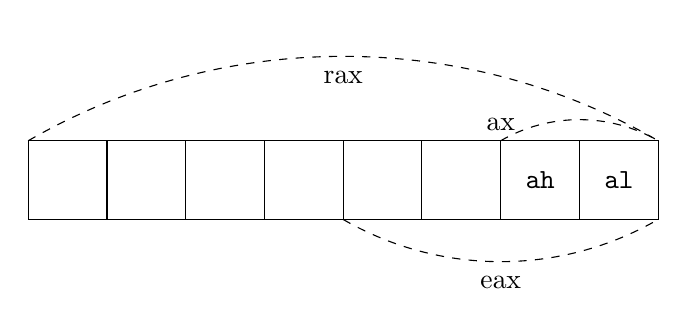
\begin{tikzpicture}
\draw (0,0) -- (8,0)  -- (8,1) -- (0,1)  --cycle;
\foreach \i in {1,...,7}{
	\draw (\i,0) -- (\i,1);
}
\draw (1,0) -- (1,1);
\draw (2,0) -- (2,1);
\draw (3,0) -- (3,1);
\node (A0) at (6.5,0.5) {\tt ah};
\node (A0) at (7.5,0.5) {\tt al}; 
\draw[dashed] (6,1) arc (120:60:2);
\draw[dashed] (4,0) arc (-120:-60:4);
\draw[dashed] (0,1) arc (120:60:8);
\node (Ax) at (6,1.2) {ax};
\node (Ax) at (6,-0.8) {eax};
\node (Ax) at (4,1.8) {rax};
\end{tikzpicture}

En d'autres termes, l'instruction \code{and eax, 0} fait passer la valeur de \code{rax} de 0x12\ 34\ 56\ 78\ 90\ ab\ cd\ ef à 0x12\ 34\ 56\ 78\ 00 00 00 00. 

Nous revenons sur certains registres en section~\ref{sec:asm}. 
 
\subsection{Instructions}

\newcommand{\Instr}{{\tt Instr}}

Les instructions sont les plus petits éléments qui pilotent le calcul. Il y a plusieurs manières de les voir. De manière abstraite, c'est un ensemble qu'on peut lister : 
\begin{eqnarray*}
&&\code{nop},\\
&&\code{add eax, ebx},\\
&&\code{mov rax, qword ptr[rcx+12]},\\
&&\code{call eax},\\
&&\ldots
\end{eqnarray*} 
Leur liste se trouve dans le manuel du constructeur du processeur. Par exemple, on retrouvera pour INTEL/x86\_64 les instructions à \cite{IntelSetInstruction}. Attention, l'ensemble des instructions varie au cours du temps, certaines apparaissent, d'autres disparaissent. Par la suite, on note $\Instr$ l'ensemble des instructions. 

Les instructions ont un codage : à chacune, on peut associer une suite d'octets : 
\begin{eqnarray*}
	\code{nop} &\mapsto& 0x90\\
	\code{add eax, ebx} &\mapsto& 0x89, 0xb8\\
	\code{mov rax, qword ptr[rcx+12]} &\mapsto&  0x67, 0x48, 0x8b, 0x41, 0x0c\\
	\code{call eax} &\mapsto& 0xff, 0xd0
	\ldots
\end{eqnarray*} 
On peut retrouver la correspondance sur plusieurs sites comme \url{https://defuse.ca/online-x86-assembler.htm}. 
 
Une \textit{instruction} se décompose selon le format\footnote{Plus de détails à \url{http://ref.x86asm.net/coder32.html} par exemple.} :%TODO dire qu'en bytes bah c'est quasiment arei
\begin{eqnarray*}
	\Instr& ::=& \code{prefix}_1 \dots \code{prefix}_k \; \code{opcode} \; \code{Arg}_1 \dots \code{Arg}_\ell\\
	\code{Arg} &::=& \code{Imm}\ |\ \Reg\ |\ \code{Mem}\\
	\label{eq3} \code{Mem} &::=& (\Seg[\Reg_1+scale*\Reg_2+\code{Disp}], size)\\ 
	\code{prefix} &:::=& {\tt rep}, {\tt lock}, {\tt data16}, \ldots\\
	\code{opcode} &::=& {\tt add}, {\tt jmp}, {\tt call}, \ldots \\
	\Seg & ::=& {\tt cs}, {\tt ds}, {\tt es}, \ldots \\
	\Reg & ::=& {\tt rax}, {\tt ebx}, \ldots
\end{eqnarray*}
où \code{Imm}, \code{Disp} désignent un immédiat (un nombre), $scale\in\{1,2,4,8\}$ et $size\in\{1, 2, 4, 8\}$. 

Le codage de l'instruction suit la structure ci-dessus : chaque préfixe est stocké sur un octet. L'opcode désigne l'opération à réaliser. Il est stocké sur un, deux ou trois octets. Ensuite, pour les arguments, les immédiats sont codés tels qu'ils apparaissent en mémoire. Les registres, registres de segments, scale et size et les références en mémoire ont un mécanisme spécifique (voir le codage \code{mod/rm}+sib). Un exemple, l'instruction $$\code{data16 adc [rbx+rcx*4+0x12],0x1357}$$
est encodée $0x66,0x81,0x54,0x8b,0x12,0x57,0x13$ : 
$$
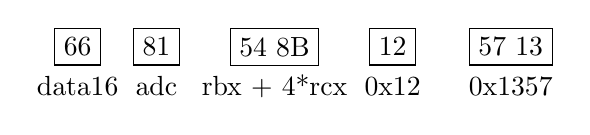
\begin{tikzpicture}
\node[draw,shape=rectangle] (A) at (0,0) {66};
\node (Aa) at (0,-0.5) {data16};
\node[draw,shape=rectangle] (B) at (1,0) {81};
\node (Ba) at (1,-0.5) {adc};
\node[draw,shape=rectangle] (C) at (2.5,0) {54 8B};
\node (Ca) at (2.5,-0.5) {rbx + 4*rcx};
\node[draw,shape=rectangle] (D) at (4,0) {12};
\node (Da) at (4,-0.5) {0x12};
\node[draw,shape=rectangle] (E) at (5.5,0) {57 13};
\node (Ea) at (5.5,-0.5) {0x1357};
\end{tikzpicture}
$$

L'encodage d'une instruction est injectif (dans les suites d'octets). A une instruction correspond un unique encodage. Par la suite, nous ne distinguons plus une instruction de son encodage.
Enfin, c'est un encodage dit préfixe :  l'encodage est tel qu'il n'y a pas deux instructions différentes dont l'encodage de l'une soit préfixe de l'autre. 

\subsection{En résumé}

L'état de la machine est donc décrite par la mémoire virtuelle et les registres. En termes mathématique, il s'agit d'un triplet $(M, \rho, R)$ désignant respectivement la valeur de chaque cellule en mémoire, les droits associés et la valeur des registres. Un tel triplet s'appelle une configuration et on note $$\Configuration = (\Addr \to \Byte) \times (\Addr \to 2^{\{R,W,X\}}) \times (\Reg \to \Byte^A)$$ 
l'ensemble de toutes les configurations. Enfin, étant donnée une configuration $C$, $M_C$ désigne la valuation de sa mémoire, $\rho_C$ ses droits et $R_C$ la valuation de ses  registres. 


 Selon l'usage, on peut "oublier" les droits en mémoire. On obtient alors un modèle moins précis mais plus simple. S'il est suffisant pour rendre compte du phénomène envisagé, il n'y a pas de raisons de se compliquer la vie. Au contraire, si on s'intéresse à l'attaque {\sc spectre}, le modèle avec valeur et droits n'est pas assez précis. Dans ce cas, il faudra rajouter des informations concernant le(s) cache. Pareil, si on doit tenir compte de l'OS--par exemple les appels systèmes, le modèle sera insuffisant. 
 
 Tout l'art consiste à trouver le bon niveau d'abstraction.
 
\section{Une sémantique opérationnelle}


L'exécution d'un programme procède de la manière suivante. A chaque étape, le processeur lit les cases mémoires $M[\rip], M[\rip+1], M[\rip+2], \ldots$ De deux choses l'une, soit un préfixe\footnote{début de la suite.} de la suite correspond à une instruction machine auquel cas celle-ci est exécutée, soit le programme est interrompu et un mécanisme d'exception prend en charge l'erreur. 

Ainsi, si la valeur de  $M[\rip]$ est $\hexa{90}$, le processeur\footnote{Pour cet exemple, et les suivants, on considère un processeur de la famille {\sc intel x86}, dans sa version 64 bits.} reconnaît l'instruction machine \code{nop} qui consiste à ne rien faire\footnote{{\tt nop} pour No OPeration. En fait, elle incrémente tout de même la valeur de \rip\ de $1$. }. Si la suite commence par $M[\eip], M[\rip+1], M[\rip+2], M[\rip+3]= \hexa{48}, \hexa{83}, \hexa{c0}, \hexa{09}$, il s'agit de l'instruction  {\tt add rax, 9} qui rajoute $9$ au registre \rax\ et passe à l'instruction suivante\footnote{C'est-à-dire incrémente \rip de $4$.}.  

Le programme  poursuit son exécution tant qu'une \emph{interruption} ne se produit pas. Les interruptions (en règle générale externes au programme en cours) peuvent apparaître à diverses occasions, une instruction illégale comme nous avons vu plus haut, une modification au niveau matériel ou bien la frappe d'une touche clavier. Suite à l'interruption, et selon une certaine politique de priorité, le système d'exploitation "reprend" la main, en d'autres termes, la valeur de \rip est modifiée directement par le processeur, en dehors du contrôle du programme. Le système rendra éventuellement la main au programme plus tard. 

Les  processeurs modernes de l'architecture {\sc x86} reconnaissent plus d'un millier d'instructions différentes. On ne les décrira pas ici. Toutefois, on pourra observer que chaque instruction lit et modifie un ou plusieurs registres, éventuellement 1, 2, 4 ou 8 octets en mémoire\footnote{\`A l'exception de certaines instructions de manipulation de chaînes comme {\tt rep stosb} qui modifient un nombre arbitraires d'octets, mais ce type d'instruction prend autant de cycles machine.}.  Il n'y a, d'une certaine manière, que huit types de données : 
\begin{itemize}
	\item 1 octet = {\tt byte}, 
	\item 2 octets = {\tt word},
	\item 4 octets = {\tt dword},
	\item 8 octets = {\tt qword},
	\item 10 octets = {\tt tword} pour les flottants en précision étendue,
	\item 16 octets = {\tt oword}, 32 = {\tt yword} et 64 {\tt zword} pour les registres spécifiques correspondant : {\tt xmm}, {\tt ymm} et {\tt zmm}
\end{itemize}

Les autres structures de données du \C, tableaux, listes, chaînes de caractères, etc sont définies à l'aide de ces briques de base.

Les instructions machine "en font le moins possible". Par exemple, pour une multiplication, il n'y a pas de vérification du type des éléments manipulés, entiers signés ou non, flottants, ni sur la taille: octet, mot, mot double ou quadruple. La machine autorise l'application  de la multiplication des flottants à un octet signé et à un mot non signé.  En d'autres termes, le programmeur doit gérer le type de chaque zone mémoire.

En conclusion, le code machine, c'est la politique des nombreux petits pas sans filets.  Les langages de plus haut niveau comme \C ou \python permettent de structurer à plus grande échelle les programmes, ils nous rapprochent de la vue algorithmique.  Pour cela, ils nous offrent essentiellement des structures de contrôle de haut niveau, un plus large éventail de données avec un typage et les outils pour les manipuler. 

\subsection{Sémantique des instructions}

Quel modèle mathématique rend compte du comportement de la machine. Ma\-thé\-matiquement, on fait l'hypothèse que l'on dispose d'une fonction $${\bf step} : \Configuration \to \Configuration$$
qui exécute une étape de calcul, c'est-à-dire une instruction machine. Cette fonction peut être décrite par la sémantique de chaque instruction séparément. Etant donnée une instruction $I$, on note 
$$\sema{I}(M,\rho, R)$$ la configuration obtenue après application de l'instruction $I$ sur la configuration $(M,\rho,R)$. 

Par conséquent, pour une configuration $C = (M,\rho, R)$,  
$${\bf step}(M,\rho,R) = \sema{I}(M,\rho,R)$$ 
où $I$ est l'instruction à l'adresse $R(\rip)$, par la suite simplifié sous la forme $\rip$ quand le contexte est clair.

 
En outre, autre hypothèse usuelle, la mémoire n'est modifiée qu'en un nombre borné de position. En d'autres termes, il existe $Mmax > 0$ tel que pour toute configuration $C$, $|\{x \in \Addr : M_{{\bf step}(C)}[x] \neq M_C[x] \}| \leq Mmax$ où $|X|$ désigne le cardinal de l'ensemble $X$.


\section{L'assembleur pour les nuls}\label{sec:asm}

Faisons un tour d'horizon de l'assembleur X86. 

\subsection{Registres}
Petit tour (incomplet) des registres. Les registres se classent en plusieurs catégories, les registres généraux sont 
$$\tt rax, rbx, rcx, rdx, rsi, rdi, r8, r9, \ldots, r15$$
ils servent à tout et à rien de particulier. Les registres $\tt rsi$ et $\tt rdi$ servent pour les instructions manipulant des chaînes de caractères. Le "s" de $\tt rsi$ vient de "source", le "d" de $\tt rdi$ pour "destination". 
Les registres
$$\tt rbp, rsp$$
sont le "base pointer" et le "stack pointer". Le registre $\tt rsp$ donne la position courante sur la pile. Le registre $\tt rbp$ donne la position en mémoire des arguments de la fonction courante. Attention, l'emploi de ces registres est conventionnel\footnote{Chercher "Application Binary Interface" sur le web.}. 
Le registre
$$\tt rip$$
désigne l'instruction courante. Le registre 
$$\tt rflags$$
contient l'état des flags. Les flags sont mis à jour pour indiquer des informations sur le calcul. Le bit 0 de $\tt rflags$ qui s'appelle $\tt cf$ pour "carry flag" indique que la dernière opération s'est terminée par une retenue (carry). Deux autres exemples de flags  : bit 6, $\tt zf$ (zero), bit 7, $\tt sf$ (signe). 

Enfin, on rencontrera les registres de segments : 
$$\tt cs, ds, ed, fs, gs, ss$$
qui ont eu une fonction importante dans le contexte des machines à addressage sur 16 bits (cs: "code segment", ds : "data segment", ss : "stack segment", etc). Ils ne sont plus employés à l'exception de {\tt fs} et {\tt gs} que nous reverrons plus tard. Ces registres sont utilisés par l'OS pour désigner des zones de mémoire pour la gestion des processus. 

\subsection{Instructions}

Commençons par les affectations. Voici un certain nombre d'instructions :  
\begin{minted}{asm}
mov rax, 0x1234     ; rax = 0x1234
mov rbx, rax        ; rbx = rax
mov rbx, [0x1234]   ; rbx = *((qword *) 0x1234)
mov ebx, [0x1234]   ; ebx = *((dword *) 0x1234) 
mov ebx, dword ptr[0x1234] ; autre forme de l'instruction précédente
mov bx, [0x1234]    ; bx = *((word *) 0x1234 )
mov bl, [0x1234]    ; bl = *((byte *) 0x1234)
mov rbx, [rax]      ; rbx = *((dword *) rax)
mov rbx, [rax+4*rcx+0x12] ; rbx = *((dword *) rax+0x12) or rbx = rax[0x12]
mov rbx, fs:[0x30]  ; rbx = [fs+0x30]
lea rax, [rbx+4*rcx+0x12] ; rax = rbx + 4*rcx + 0x12
\end{minted}

Quelques opérations arithmétiques : 
\begin{minted}{asm}
xor eax, eax    ; eax ^= eax or eax = 0
add rax, rbx    ;  rax += rbx
sub rax, 0x12   ; rax -= 0x12
imul rax, [rbx] ; signed mul, rax *= [0x12] seen as qword 
imul rbx        ; rax *= rbx (rax is implicit) 
mul rbx         ; unsigned mul, rax *= rbx 
fmul [rsp+8]    ; floating point multiplication (st(0) is implicit)
idiv  [0x1234]  ; ah = rax / *(0x1234), al = rax % *(0x1234)
\end{minted}
Ces opérations vont mettre à jour le registre des flags (carries, zero, etc). Mise à jour des flags,
\begin{minted}{asm}
cmp rax, rbx    ; ZF == (rax - rbx == 0), SF == (rax - rbx > 0)
cmp rax, 0x12   ; 
test rax, rbx   ; ZF == (rax & rbx == 0)
\end{minted}


Opérations sur la pile : 
\begin{minted}{asm}
push eax        ; empilement
pop rbx         ; dépilement
push 0x12       ; empilement de 8 octets (avec des zeros)
pushf           ; "push rflags"
popf            ; "pop rflags"  
\end{minted}

Instructions de contrôle (où next\_ins désigne l'adresse de l'insruction suivante) : 
\begin{minted}{asm}
jmp 0x1234      ; rip = 0x1234 <=> goto 0x1234
jmp [0x1234]    ; rip = [0x1234]
jmp rax         ; rip = rax
jmp [rax]       ; rip = *rax
jz 0x1234       ; si ZF rip = 0x1234 sinon rip = next_ins
; jnz (not zero), jle (lower or equal), jg (greater), etc
\end{minted}

Appels de fonctions
\begin{minted}{asm}
call 0x1234 ; push next_ins; rip = 0x1234
ret         ; pop rip
call rbx
call [rax+0x12]
call [0x1234]
leave       ; rsp = rbp, pop rbp
\end{minted}

Interruptions
\begin{minted}{asm}
int3        ; interruption, utilisée par le debugger
\end{minted}

\chapter{De la machine au programme}

Lorsqu'on double-clique sur un programme, il est exécuté. Dans ce chapitre, on va voir ce qui se passe plus en détails. 

\section{Le programme en mémoire}

Dans un premier temps, observons la structure de la mémoire au démarrage du programme. Les expériences sont présentées en \C sous Windows. Pour Linux, il y a pleins de variations, mais on retrouve assez rapidement les analogies. Compilons le programme suivant : 

\begin{minted}{C}
#include <stdio.h>
#include <stdlib.h>
char a ='A',b='B';
int main(int argc, char *argv[]){
	int i = 42, j;
	int *p =(int *) malloc(sizeof(int));
	printf("[%p] = %d\n", &i, i);
	printf("[%p] = %c\n", &a, a);
	printf("[%p] = %x\n", p, *p);
	return 0;
}
\end{minted}

Il y a quatre grandes zones de mémoire visibles (avec un des droits R, W, X) à l'utilisateur : 
\begin{itemize}
	\item le programme lui-même,
	\item la pile,
	\item le tas,
	\item la zone des bibliothèques partagées (DLLs).
\end{itemize}

La pile contient typiquement : les variables locales des fonctions (\code{i, j}), les retours des fonctions. Le tas contient toutes les données allouées dynamiquement, avec un malloc. Le programme va contenir les instructions (\code{main}), les variables globales (\code{a},\code{b}), et différentes ressources (icones, etc). Enfin, les DLLs ont la même structure que l'exécutable lui-même (\code{msvcrt.dll} qui contient le code de \code{printf}). Elles vont avoir leur propre pile, leur propre tas, etc. 



\chapter{Obfuscations}

\section{Cacher l'appel de la fonction}

L'utilisation de fonctions, en particulier celles provenant des bibliothèques, donne bien sûr beaucoup d'informations sur ce que fait le programme. C'est la raison pour laquelle l'appel des fonctions est généralement obfusqué. On propose quelques techniques dans cette section. 











\bibliographystyle{alpha}

\bibliography{references}	
\end{document}